\documentclass[modern]{aastex62}

\usepackage{units}

\newcommand{\MESA}{{\tt MESA}}

% define some useful commands
\newcommand{\Msun}{\ensuremath{\mathrm{M}_\odot}}
\newcommand{\gcc}{\ensuremath{\mathrm{g\,cm^{-3}}}} % density units

\newcommand{\Mch}{\ensuremath{\mathrm{M}_{\rm Ch}}}

\newcommand{\Ye}{\ensuremath{Y_{\rm e}}}
\newcommand{\EF}{\ensuremath{E_{\rm F}}}

% central quantities
\newcommand{\Tc}{\ensuremath{T_{\rm c}}}
\newcommand{\Rhoc}{\ensuremath{\rho_{\rm c}}}

\newcommand{\epsnu}{\ensuremath{\epsilon_{\nu}}} % Neutrino loss rate
\newcommand{\epsnuc}{\ensuremath{\epsilon_{\mathrm{nuc}}}} % Neutrino loss rate


% nuclides.tex
% input file with macros for nuclides

% base command
\newcommand{\nuclei}[2]{\ensuremath{\mathrm{^{#1}#2}}}

% nuclides, with most highest abundance or longest half-life as default
% for example, \carbon produces ^{12}C, \carbon[13] produces ^{13}C
%
\newcommand{\hydrogen}[1][1]{\nuclei{#1}{H}}
\newcommand{\helium}[1][4]{\nuclei{#1}{He}}
\newcommand{\lithium}[1][7]{\nuclei{#1}{Li}}
\newcommand{\beryllium}[1][9]{\nuclei{#1}{Be}}
\newcommand{\boron}[1][11]{\nuclei{#1}{B}}
\newcommand{\carbon}[1][12]{\nuclei{#1}{C}}
\newcommand{\nitrogen}[1][14]{\nuclei{#1}{N}}
\newcommand{\oxygen}[1][16]{\nuclei{#1}{O}}
\newcommand{\fluorine}[1][19]{\nuclei{#1}{F}}
\newcommand{\neon}[1][20]{\nuclei{#1}{Ne}}
\newcommand{\sodium}[1][23]{\nuclei{#1}{Na}}
\newcommand{\magnesium}[1][24]{\nuclei{#1}{Mg}}
\newcommand{\aluminum}[1][27]{\nuclei{#1}{Al}}
\newcommand{\silicon}[1][28]{\nuclei{#1}{Si}}
\newcommand{\phosphorus}[1][31]{\nuclei{#1}{P}}
\newcommand{\sulfur}[1][32]{\nuclei{#1}{S}}
\newcommand{\chlorine}[1][35]{\nuclei{#1}{Cl}}
\newcommand{\argon}[1][36]{\nuclei{#1}{Ar}}
\newcommand{\potassium}[1][39]{\nuclei{#1}{K}}
\newcommand{\calcium}[1][40]{\nuclei{#1}{Ca}}
\newcommand{\scandium}[1][45]{\nuclei{#1}{Sc}}
\newcommand{\titanium}[1][48]{\nuclei{#1}{Ti}}
\newcommand{\vanadium}[1][51]{\nuclei{#1}{V}}
\newcommand{\chromium}[1][52]{\nuclei{#1}{Cr}}
\newcommand{\manganese}[1][55]{\nuclei{#1}{Mn}}
\newcommand{\iron}[1][56]{\nuclei{#1}{Fe}}
\newcommand{\cobalt}[1][59]{\nuclei{#1}{Co}}
\newcommand{\nickel}[1][58]{\nuclei{#1}{Ni}}
\newcommand{\copper}[1][63]{\nuclei{#1}{Cu}}
\newcommand{\zinc}[1][64]{\nuclei{#1}{Zn}}
\newcommand{\gallium}[1][69]{\nuclei{#1}{Ga}}
\newcommand{\germanium}[1][74]{\nuclei{#1}{Ge}}
\newcommand{\arsenic}[1][75]{\nuclei{#1}{As}}
\newcommand{\selenium}[1][80]{\nuclei{#1}{Se}}
\newcommand{\bromine}[1][79]{\nuclei{#1}{Br}}
\newcommand{\krypton}[1][84]{\nuclei{#1}{Kr}}
\newcommand{\rubidium}[1][85]{\nuclei{#1}{Rb}}
\newcommand{\strontium}[1][88]{\nuclei{#1}{Sr}}
\newcommand{\yttrium}[1][89]{\nuclei{#1}{Y}}
\newcommand{\zirconium}[1][94]{\nuclei{#1}{Zr}}
\newcommand{\niobium}[1][93]{\nuclei{#1}{Nb}}
\newcommand{\molybdenum}[1][98]{\nuclei{#1}{Mo}}
\newcommand{\technetium}[1][97]{\nuclei{#1}{Tc}}
\newcommand{\ruthenium}[1][102]{\nuclei{#1}{Ru}}
\newcommand{\rhodium}[1][103]{\nuclei{#1}{Rh }}
\newcommand{\palladium}[1][106]{\nuclei{#1}{Pd}}
\newcommand{\silver}[1][107]{\nuclei{#1}{Ag}}
\newcommand{\cadmium}[1][114]{\nuclei{#1}{Cd}}
\newcommand{\indium}[1][115]{\nuclei{#1}{In}}
\newcommand{\tin}[1][120]{\nuclei{#1}{Sn}}
\newcommand{\antimony}[1][121]{\nuclei{#1}{Sb}}
\newcommand{\tellurium}[1][130]{\nuclei{#1}{Te}}
\newcommand{\iodine}[1][127]{\nuclei{#1}{I}}
\newcommand{\xenon}[1][132]{\nuclei{#1}{Xe}}
\newcommand{\cesium}[1][133]{\nuclei{#1}{Cs}}
\newcommand{\barium}[1][138]{\nuclei{#1}{Ba}}
\newcommand{\lanthanum}[1][139]{\nuclei{#1}{La}}
\newcommand{\cerium}[1][140]{\nuclei{#1}{Ce}}
\newcommand{\praseodymium}[1][141]{\nuclei{#1}{Pr}}
\newcommand{\neodymium}[1][142]{\nuclei{#1}{Nd}}
\newcommand{\promethium}[1][147]{\nuclei{#1}{Pm}}
\newcommand{\samarium}[1][152]{\nuclei{#1}{Sm}}
\newcommand{\europium}[1][153]{\nuclei{#1}{Eu}}
\newcommand{\gadolinium}[1][158]{\nuclei{#1}{Gd}}
\newcommand{\terbium}[1][159]{\nuclei{#1}{Tb}}
\newcommand{\dysprosium}[1][164]{\nuclei{#1}{Dy}}
\newcommand{\holmium}[1][165]{\nuclei{#1}{Ho}}
\newcommand{\erbium}[1][168]{\nuclei{#1}{Er}}
\newcommand{\thulium}[1][169]{\nuclei{#1}{Tm}}
\newcommand{\ytterbium}[1][174]{\nuclei{#1}{Yb}}
\newcommand{\lutetium}[1][175]{\nuclei{#1}{Lu}}
\newcommand{\hafnium}[1][180]{\nuclei{#1}{Hf}}
\newcommand{\tantalum}[1][180]{\nuclei{#1}{Ta}}
\newcommand{\tungsten}[1][184]{\nuclei{#1}{W}}
\newcommand{\rhenium}[1][187]{\nuclei{#1}{Re}}
\newcommand{\osmium}[1][192]{\nuclei{#1}{Os}}
\newcommand{\iridium}[1][193]{\nuclei{#1}{Ir}}
\newcommand{\platnium}[1][195]{\nuclei{#1}{Pt}}
\newcommand{\gold}[1][197]{\nuclei{#1}{Au}}
%\newcommand{\mercury}[1][202]{\nuclei{#1}{Hg}}
\newcommand{\thallium}[1][205]{\nuclei{#1}{Tl}}
\newcommand{\lead}[1][208]{\nuclei{#1}{Pb}}
\newcommand{\bisumth}[1][209]{\nuclei{#1}{Bi}}
\newcommand{\polonium}[1][208]{\nuclei{#1}{Po}}
\newcommand{\astatine}[1][219]{\nuclei{#1}{At}}
\newcommand{\radon}[1][222]{\nuclei{#1}{Rn}}
\newcommand{\francium}[1][223]{\nuclei{#1}{Fr}}
\newcommand{\radium}[1][226]{\nuclei{#1}{Ra}}
\newcommand{\actinium}[1][227]{\nuclei{#1}{Ac}}
\newcommand{\thorium}[1][232]{\nuclei{#1}{Th}}
\newcommand{\protactinium}[1][231]{\nuclei{#1}{Pa}}
\newcommand{\uranium}[1][238]{\nuclei{#1}{U}}
\newcommand{\neptunium}[1][237]{\nuclei{#1}{Np}}
\newcommand{\plutonium}[1][244]{\nuclei{#1}{Pu}}
\newcommand{\americium}[1][243]{\nuclei{#1}{Am}}
\newcommand{\curium}[1][248]{\nuclei{#1}{Cm}}
\newcommand{\berkelium}[1][247]{\nuclei{#1}{Bk}}
\newcommand{\californium}[1][251]{\nuclei{#1}{Cf}}
\newcommand{\einsteinium}[1][252]{\nuclei{#1}{Es}}
\newcommand{\fermium}[1][257]{\nuclei{#1}{Fm}}
\newcommand{\mendelevium}[1][260]{\nuclei{#1}{Md}}
\newcommand{\nobelium}[1][259]{\nuclei{#1}{No}}
\newcommand{\lawrencium}[1][262]{\nuclei{#1}{Lr}}
\newcommand{\rutherfordium}[1][261]{\nuclei{#1}{Rf}}
\newcommand{\dubnium}[1][262]{\nuclei{#1}{Db}}
\newcommand{\seaborgium}[1][266]{\nuclei{#1}{Sg}}
\newcommand{\bohrium}[1][267]{\nuclei{#1}{Bh}}
\newcommand{\hassium}[1][269]{\nuclei{#1}{Hs}}
\newcommand{\meitnerium}[1][268]{\nuclei{#1}{Mt}}
\newcommand{\darmstadtium}[1][271]{\nuclei{#1}{Ds}}


\usepackage{amsmath}

\begin{document}

% \author[0000-0002-4870-8855]{Josiah Schwab}
% \altaffiliation{Hubble Fellow}
% \affiliation{Department of Astronomy and Astrophysics, University of California, Santa Cruz, CA 95064, USA}
% \correspondingauthor{Josiah Schwab}
% \email{jwschwab@ucsc.edu}

% \title{}

\section{Relevant Timescales}

We define the accretion timescale as
\begin{equation}
  t_{\mathrm{accrete}} = \frac{M}{\dot{M}}
\end{equation}
and the compression timescale as
\begin{equation}
  \label{eq:tcompress}
  t_{\mathrm{compress}} = \left(\frac{d \ln \rho}{dt} \right)^{-1}~.
\end{equation}
The central density rises rapidly as one approaches the Chandrasekhar
mass and therefore the compression timescale is significantly shorter
than the accretion timescale (by a factor $\sim 100$).


We define the electron-capture timescale as
\begin{equation}
  \label{eq:tcapture}
  t_{\mathrm{capture}} = \left(\frac{d \ln \Ye}{dt} \right)^{-1}
\end{equation}
and the heating timescale as
\begin{equation}
  \label{eq:cooling}
  t_{\mathrm{heat}} = \frac{c_P T}{\epsnuc} ~.
\end{equation}
We will primarily be interested in the exothermic electron captures,
but we will plot the absolute value of this quantity so that it
represents the cooling timescale at times when the Urca-process is
operating.


For the plots of these timescales in previous work on ECSN
progenitors, see Figure 7 in \citet{Miyaji1980}, Figure 2 in
\citet{Miyaji1987}, and Figure 9 in \citet{Takahashi2013}.

The figures show these timescales for for an ONe WD accreting at
$\dot{M} = 10^{-6}\,\Msunyr$.  Two WD models are shown: SQB15 is the
fiducial model used in \citet{Schwab2015}, which has only even-A
isotopes (\oxygen[16], \neon[20], \magnesium[24]); SBQ17 is the
fiducial model used in \citet{Schwab2017a}, which also includes the
odd-A isotopes \sodium[23] and \magnesium[25] and experiences
significant Urca-process cooling.  Table 1 gives the detailed
compositions.  We show a run using the ``on-the-fly'' rates in \MESA\
assuming only allowed transitions contribute and another run assuming
the non-unique second forbidden transitions have
$\log(ft) \approx 11$.  We also show the results of using the
\citet{Suzuki2016a} tables.  In these tables, the relevant non-unique
second forbidden transition for \neon[20] is at the (previous)
experimental upper limit.

The models in Figure 3 all want to convect around the time of the
$A=24$ electron captures, but in these runs we have artificially
suppressed convection.  (Once the models become convective in this
regime, \MESA\ struggles for a variety of reasons.)

The \MESA\ models all halt at oxygen ignition.  The heating/capture
timescales will naturally continue to decrease beyond this point.


\begin{table}
  \centering
  \caption{The set of compositions used in our \MESA\ models.  Each
    composition is referenced in the text by the identifier listed in
    the top row.  Each column lists the mass fractions of the isotopes
    (listed at left) that were included.  Dashes indicate that a
    particular isotope was not included.}
  \label{tab:compositions}
  \begin{tabular}{rcc}
    \hline
    Isotope & SQB15 & SBQ17 \\
    \hline
    \oxygen[16]    & 0.500 & 0.500 \\
    \neon[20]      & 0.450 & 0.390 \\
    \neon[22]      & ---   & ---   \\
    \sodium[23]    & ---   & 0.050 \\
    \magnesium[24] & 0.050 & 0.050 \\
    \magnesium[25] & ---   & 0.010 \\
    \hline
  \end{tabular}
\end{table}

\begin{figure}
  \centering
  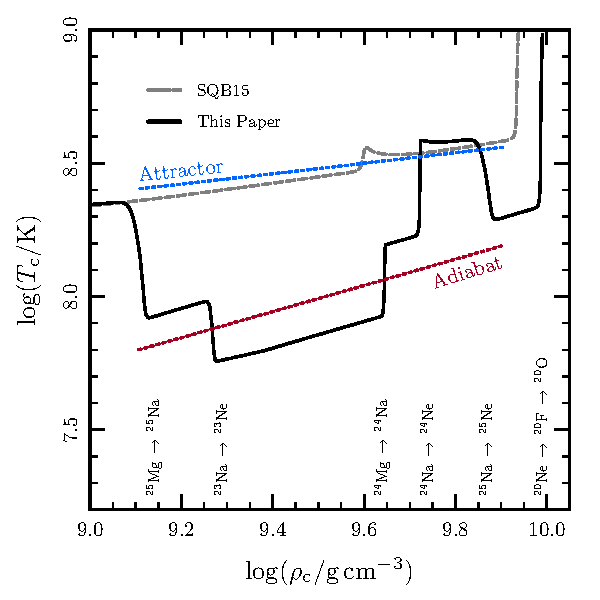
\includegraphics[width=\textwidth]{schematic.pdf}
  \caption{Central density-temperature evolution for of the accreting
    WD models with the effects of various reactions labeled. (This is
    Figure 5 in \citealt{Schwab2017a}.)}
\end{figure}

\begin{figure}
  \centering
  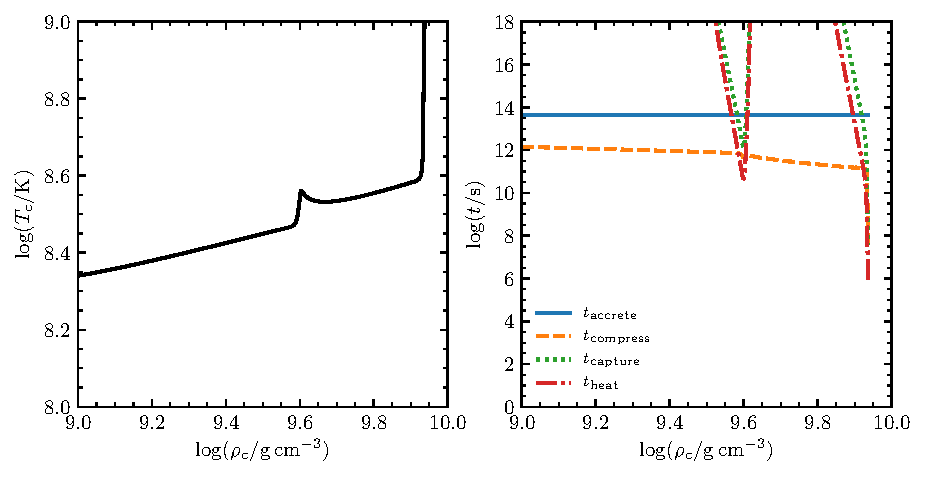
\includegraphics[width=0.95\textwidth]{SQB15-allowed.pdf}
  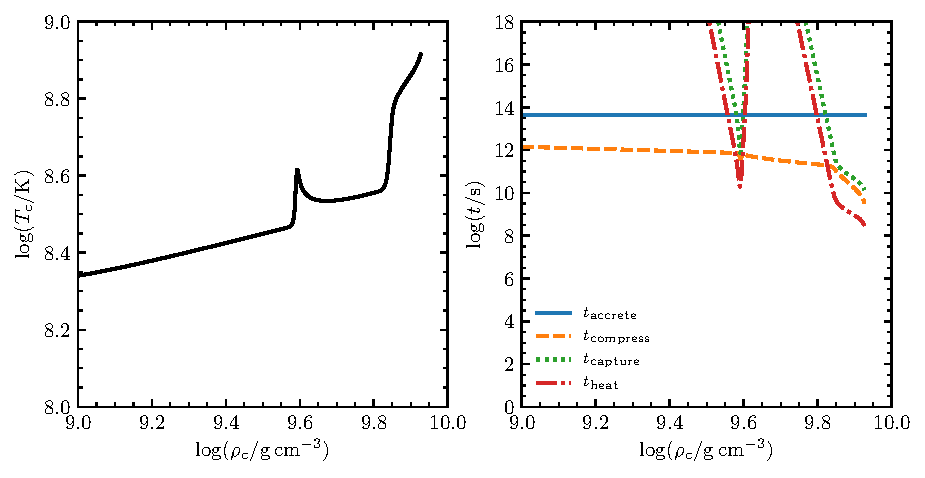
\includegraphics[width=0.95\textwidth]{SQB15-nusf11.pdf}
  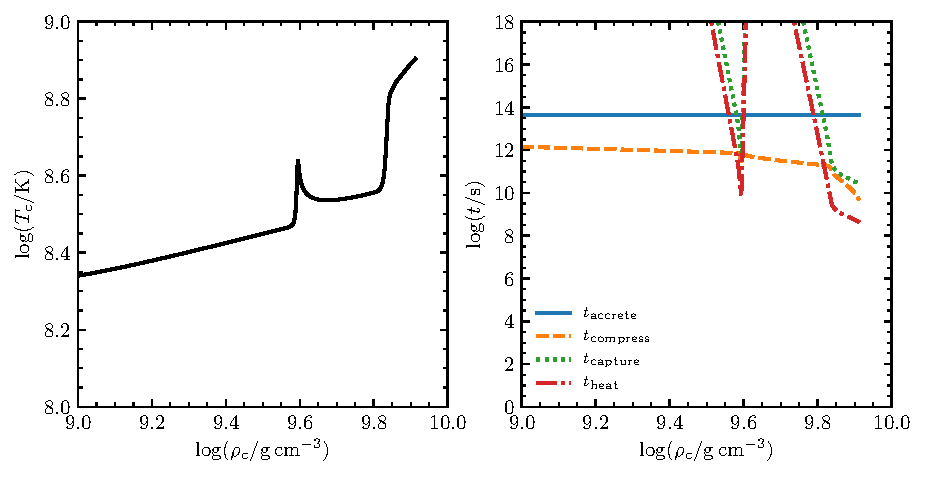
\includegraphics[width=0.95\textwidth]{SQB15-suzuki.pdf}

  \caption{Evolution without Urca-process cooling (SQB15 model).  \textit{Upper panel}: On-the-fly rates with allowed transitions only;  \textit{Middle panel}: On-the-fly rates including non-unique second forbidden transitions; \textit{Lower panel}: \citet{Suzuki2016a} rate tables. \label{fig:SQB15}}
\end{figure}

\begin{figure}
  \centering
  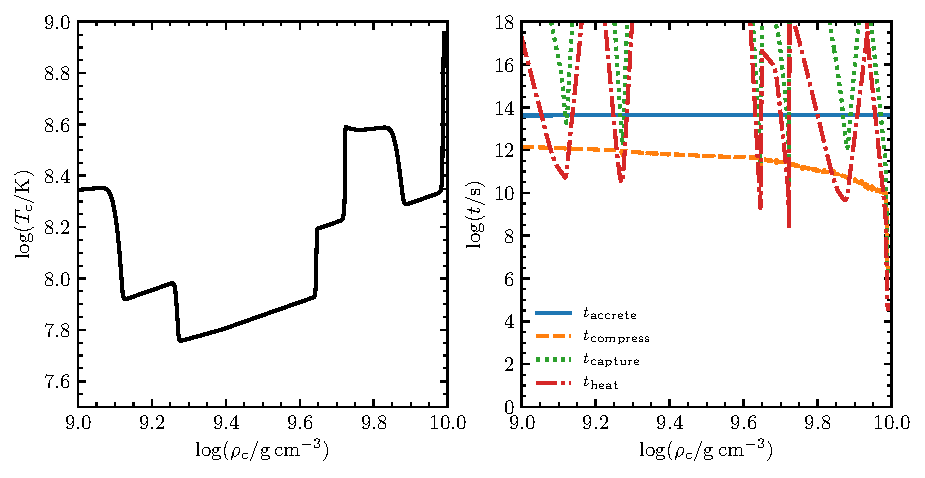
\includegraphics[width=0.95\textwidth]{SBQ17-allowed.pdf}
  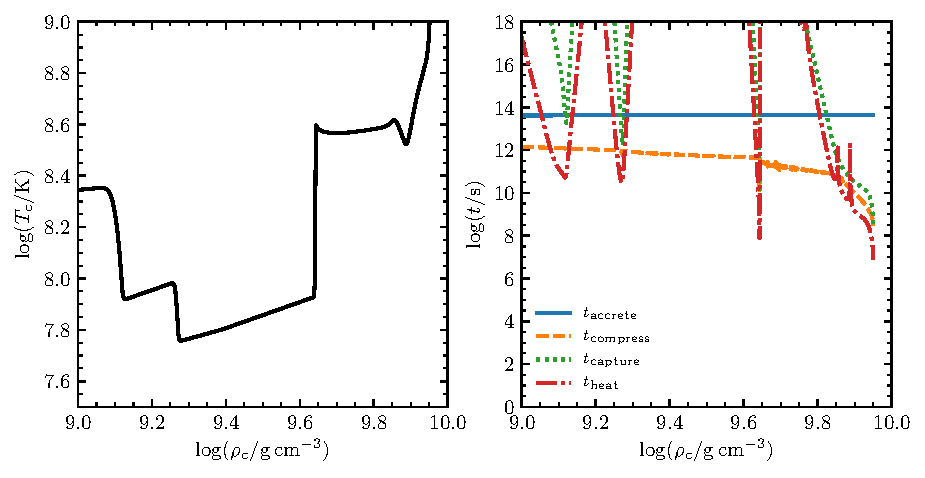
\includegraphics[width=0.95\textwidth]{SBQ17-nusf11.pdf}
  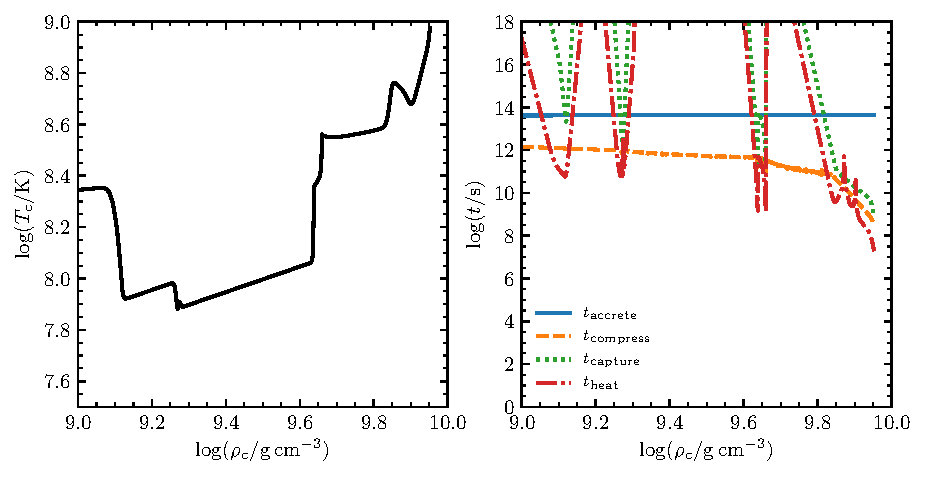
\includegraphics[width=0.95\textwidth]{SBQ17-suzuki.pdf}
  \caption{Evolution with Urca-process cooling (SBQ17 model). \textit{Upper panel}: On-the-fly rates with allowed transitions only;  \textit{Middle panel}: On-the-fly rates including non-unique second forbidden transitions; \textit{Lower panel}: \citet{Suzuki2016a} rate tables. \label{fig:SBQ17}}
\end{figure}

\newpage
~
\newpage

\section{Evolution to Oxygen Ignition}

We decided (at least initially) to focus on oxygen ignition.  We will
use the \citet{Suzuki2016a} rate tables and thus operate under the
assumption that the strength of the non-unique second forbidden
transition of $\neon[20] \to \fluorine[20]$ is around the value
adopted therein.  As mentioned by \citet{Schwab2015}, and discussed in
somewhat more detail by \citet{Moller2017}, the inclusion of this
transition leads to off-center oxygen ignition.  (In contrast, models
that omit this transition, or assume its strength is far below the
experimental upper limit, show central ignitions.)  This may be
important in understanding the subsequent evolution and final outcome.


As is pointed out by \citet{Moller2017}, including the forbidden
transition also significantly changes the elapsed time between the
onset of \neon[20] captures and the beginning of oxygen burning.  For
example, the model in the upper panel of Figure~\ref{fig:SQB15}
(allowed transitions only) takes about $\sim \unit[1]{yr}$ versus the
model in the lower panel \citep[tables from][]{Suzuki2016a} which
takes $\sim \unit[100]{yr}$\footnote{\citet{Moller2017} quotes
  timescales of a few years and a few days respectively.  We're
  probably just measuring differently; at any rate, the ratio is about
  the same.}.  It's not clear that's of importance for the evolution
-- though it does allow more time for oscillatory double diffusive
convection to operate -- but for our hydrodynamics calculations, it
just means that we really can't start near the onset of neon captures.


To understand the evolution towards an off-center ignition in more
detail, and since the goal is to provide simple initial conditions for
hydrodynamics calculations, we evolve a pure oxygen-neon WD model.
Fiducially, we select mass fractions 60\% \oxygen[16] and 40\%
\neon[20], but we will demonstrate the effect of varying the \neon[20]
fraction.  Figure~\ref{fig:ONe6040} shows the evolution of the
fiducial model.  The left plot shows the evolution of the center and
the location of the maximum rate of nuclear energy release in the
$T-\rho$ plane.  In the right plot, the upper panel shows a series of
temperature profiles. The line colors match the dots in the left plot;
one can see the evolution as the hot spot moves off center.  The final
off-center ignition at $r \approx \unit[70]{km}$ is evident in the
sharply peaked teal line.\footnote{This is in agreement with the
  models of \citet{Moller2017}, which found ignitions
  $\approx \unit[50]{km}$ off center.}  The lower panel shows the
\neon[20] profiles.  Note that the model experiences nearly-complete
neon depletion by the time of ignition.  This is in contrast to the
calculation excluding the forbidden transition, where only
$\approx 10\%$ of the \neon[20] is consumed \citep[see Figure 5
in][]{Schwab2015}.  This means the central
$M \sim \unit[5 \times 10^{-3}]{\Msun}$ is almost pure \oxygen[16] and
\oxygen[20] with a low $\Ye \approx 0.46$.

\begin{figure}
  \centering
  \includegraphics[width=0.49\textwidth]{ONe6040-RhoT.pdf}
  \includegraphics[width=0.49\textwidth]{ONe6040-profiles.pdf}
  \caption{Evolution of fiducial pure ONe WD model.  \textit{Left
      panel}: Temperature-density evolution.  The solid line shows the
    central $T$ and $\rho$; the dotted line shows the $T$ and $\rho$
    at the location of the maximum rate of nuclear energy release.
    The separation indicates the WD is evolving towards off-center
    ignition.  \textit{Right panel}: Profiles (as a function of
    radius) of the temperature (upper plot) and \neon[20] mass
    fraction (lower plot).  The matching colored dot in the left panel
    indicates the conditions at the time of each profile.}
  \label{fig:ONe6040}
\end{figure}


We now provide a more complete description of how and why this
off-center ignition occurs.  At first, the \neon[20] thermal runaway
proceeds quite similarly, except for the fact that it begins at the
lower threshold density associated with the forbidden transition
$\logRho \approx 9.8$, versus the $\logRho \approx 9.95$ threshold
density for the allowed transition.  While the conditions are
sub-threshold, the rate increases exponentially with temperature and
density.  However, near threshold, this becomes a much more gentle,
power-law rise.  Thus, in conditions where the forbidden transition
dominates, but before the allowed transition kicks in around its
threshold density, the electron capture rate tops out around
$\lambda_{\rm ec} \sim \unit[10^{-8}]{s}$ \citep[see Figure 1 in
][]{MartinezPinedo2014}.


This implies that the rate of nuclear energy release from the
\neon[20] electron captures no longer rises rapidly with temperature.
In turn, because thermal neutrino losses do rise rapidly with
increasing temperature, there exists is a temperature where heating
from electron captures and cooling from thermal neutrino losses can
balance.  Because of the relatively slow electron capture rate, this
temperature is \textit{below} the temperature at which oxygen burns.
As a result, the runaway halts, and the center of the star moves into
a phase where it satisfies a balanced-power condition
$\epsnuc \approx \epsnu$.  The fact that the center can achieve this
balance then precludes a central ignition.\footnote{In support of this
  point, we turn off thermal neutrino losses in \MESA\ and confirm
  that doing so does lead to a central ignition.}

% add something about why it is off-center

Figure~\ref{fig:ONe-vary} shows the results of a set of calculations
varying the \neon[20] mass fraction.  The left panel shows the
$T-\rho$ evolution, as in Figure~\ref{fig:ONe6040}.  The central
temperature evolution is notably different in the three cases, but the
evolution at the location of the peak of $\epsnuc$ is not.  The right
panel shows the logarithm of the ratio of $\epsnuc$ to $\epsnu$ at the
center of the WD.  Note that after the initial runaway, this has a
value $\approx 0$, demonstrating our earlier assertion that nuclear
energy generation and thermal neutrino losses are balanced.  The
$X_{\rm Ne} = 0.3$ case deviates from this balance near the end, after
it exhausts its \neon[20].

\begin{figure}
  \centering
  \includegraphics[width=0.49\textwidth]{ONe-RhoT.pdf}
  \includegraphics[width=0.49\textwidth]{ONe-epsratio.pdf}
  \caption{Comparison of models with varying \neon[20] fractions.
    \textit{Left Panel}: Temperature-density evolution.  As in
    Figure~\ref{fig:ONe6040}, the solid line shows the central $T$ and
    $\rho$; the dotted line shows the $T$ and $\rho$ at the location
    of the maximum rate of nuclear energy release.  \textit{Right
      Panel}: Ratio of the nuclear energy generation rate to the
    thermal neutrino cooling rate, evaluated at the center of the WD.}
  \label{fig:ONe-vary}
\end{figure}


The fact that the $T-\rho$ evolution at the location that runs away is
roughly independent of the \neon[20] fraction (left panel of
Figure~\ref{fig:ONe-vary}) fits into this picture.  In particular, the
location that runs away is the first place that is able to get
electron captures that can go fast enough to overcome the neutrino
losses around the oxygen ignition temperature.  Since the runaway
doesn't complete in the center, that does mean that some extra heat is
conducted into the surrounding layers.  But I'm not sure that helps
much; it doesn't matter if you get hotter if you then radiate it away
via neutrinos.  Instead, I think the most important thing is that the
layers surrounding the center get denser as the center \Ye\ falls and
it contracts.  Once this material gets a bit closer to the threshold
density for the allowed transition, when it gets hot, the allowed
transition can begin to dominate the rate \citep[again, see Figure 1
in ][]{MartinezPinedo2014}.  If that's the right picture, then I think
that predicts that higher \neon[20] fractions (which can evolve to
lower $\Ye$), should experience ignition less off-center.
Table~\ref{tab:ONe-ignition} appears to indicate that is the case.

\begin{table}
  \centering
  \caption{Location of ignition as a function of \neon[20] mass
    fraction.}
  \label{tab:ONe-ignition}
  \begin{tabular}{cc}
    \hline
    $X_{\rm Ne}$ & Ignition \\
     & [km] \\
    \hline
    0.3 & 85 \\
    0.4 & 73\\
    0.5 & 65 \\
    \hline
  \end{tabular}
\end{table}


\bibliography{timescales.bib}


\end{document}

%%% Local Variables:
%%% mode: latex
%%% TeX-master: t
%%% End:
